\documentclass[8pt,landscape]{article}

% PACKAGES
\usepackage[letterpaper, margin=0.1in]{geometry}
\usepackage{amsmath, amssymb, geometry}
\usepackage{multicol}
\usepackage{setspace}
\usepackage{sectsty}
\usepackage{verbatim}
\usepackage{graphicx}
\usepackage{xcolor}
\usepackage{listings}
\usepackage{enumitem}
\usepackage{booktabs} % For better tables if needed

% Define a custom color for code highlighting and environment
\definecolor{myred}{RGB}{204, 0, 0} % A strong red
\definecolor{mygray}{RGB}{240, 240, 240} % Light gray for background

\setlist[itemize,enumerate]{
    noitemsep,
    topsep=0pt,
    partopsep=0pt,
    parsep=0pt,
    leftmargin=*,
    labelsep=0.5em,
}

% LISTINGS SETUP for R and Python
\lstset{
  basicstyle=\ttfamily\scriptsize\color{black}, % Tiny font for code
  backgroundcolor=\color{mygray},
  frame=single,
  frameround=tttt,
  framesep=3pt,
  rulesepcolor=\color{black!20},
  breaklines=true,
  columns=fullflexible,
  showstringspaces=false,
  commentstyle=\color{gray},
  keywordstyle=\color{blue!80!black},
  stringstyle=\color{myred}, % Use red for strings to match the custom \code{} style
  breakatwhitespace=true,
  xleftmargin=0pt,
  xrightmargin=0pt,
  aboveskip=0pt,
  belowskip=0pt
}

% FORMATTING
\setstretch{0.8} % Reduce line spacing
\setlength{\parindent}{0pt}
\setlength{\parskip}{0pt}

\makeatletter

% --- Redefine Sections (Red, 8pt) ---
\renewcommand{\section}{\@startsection{section}{1}{0pt}%
    {-0.5ex}% space before (minimal, no indent)
    {0.1ex}% space after (nearly zero)
    {\fontsize{8}{9}\bfseries\color{red}}}

% --- Redefine Subsections (Blue, 8pt) ---
\renewcommand{\subsection}{\@startsection{subsection}{2}{0pt}%
    {-0.4ex}% space before (even tighter than section)
    {0.1ex}% space after
    {\fontsize{8}{9}\bfseries\color{blue}}}

\makeatother

% Custom command for red-highlighted code/commands (for in-line use)
\newcommand{\code}[1]{\textcolor{myred}{\texttt{#1}}}

% Custom small text wrapper - ensuring 8pt for body text
\newcommand{\smalltext}[1]{%
  {\fontsize{8}{9}\selectfont\sloppy #1\par}%
}

% DOCUMENT START
\begin{document}
\fontsize{8}{9}\selectfont % Set the base font size to 8pt and line skip to 9pt for the entire document
\pagestyle{empty}
\begin{multicols}{3}

\section{Training NN}
\begin{lstlisting}[language=Python]
model = models.densenet121(weights='DenseNet121_Weights.DEFAULT')
for param in model.parameters():  
    param.requires_grad=False#Freeze params so we don't update them
def trainer(model,criterion,optimizer,train,valid,epochs=5,patience=5):
    train_loss, valid_loss, val_acc = [], [], []
    for epoch in range(epochs):  # Loop over the number of epochs
        train_batch_loss = 0  # get training loss of current epoch
        valid_batch_loss = 0  # get validation loss of current epoch
        valid_batch_acc = 0   # get validation acc of current epoch
        # Training loop
        for X, y in train:  # Loop training data in batches
            optimizer.zero_grad()# Clear previous gradients
            y_hat = model(X)# Forward pass thru model to get pred
            loss=criterion(y_hat,y)#Get loss btw pred and true labels
            loss.backward()#backpropagation to calculate gradients
            optimizer.step()# Update model param based on gradients
            train_batch_loss += loss.item()  # Get the loss for batch
        train_loss.append(train_batch_loss / len(train))  #Compute avg train loss for the epoch
        # Validation Loop 
        with torch.no_grad():  #Disable gradient computation(saves memory and speeds up evaluation)
            for X, y in valid: # Loop valid data in batches
                y_hat = model(X)#Forward pass thru model to get pred
                _, y_hat_labels = torch.softmax(y_hat, dim=1).topk(1, dim=1)  # get pred class labels
                loss = criterion(y_hat, y)#Compute lossfor validbatch
                valid_batch_loss += loss.item()#Gather loss for batch
                # Compute batch accuracy by comparing pred-truelabels
                valid_batch_acc += (y_hat_labels.squeeze() == y).type(torch.float32).mean().item()
        # Compute average validation loss and accuracy for epoch
        valid_loss.append(valid_batch_loss / len(valid))
        val_acc.append(valid_batch_acc / len(valid))
    results = {"TR L":train_loss,"VL L":valid_loss,"VL ACC":val_acc}
    return results
criterion = nn.CrossEntropyLoss() 
optimizer = optim.Adam(model.parameters())
results = trainer(model, criterion, optimizer, train, valid)
\end{lstlisting}

\subsection{Differentiation}
\smalltext{
\textbf{Symbolic differentiation:} analytical derivation or “do it by hand”.
\textbf{Numerical differentiation:} using finite difference $\frac{df}{dx} \approx \frac{f(x+h)-f(x)}{h}$
\textbf{Automatic differentiation:} breaking down computations into elementary sequential steps, and using the chain rule.
Backpropagation is to use these results to easily calculate derivatives earlier in the network using the chain rule. \\
1. Forward pass: compute outputs and loss.\\
2. Backward pass: compute gradients of the loss wrt parameters. 
The gradient signal flows from loss to earlier layers. So first layer gradients are calculated last. Hence the backpropogation term!
We do this using \textbf{Autograd} PyTorch's automatic differentiation engine
}
\subsection{Vanishing/Exploding Gradients}
\smalltext{
The backpropagation algorithm uses the chain rule to compute the gradients.
The chain rule involves multiplying potentially many terms together which prevents the model from learning\\
Activations saturate (sigmoid/tanh at large |x| the derivative is close to 0) \\
ReLU helps because for positive inputs, derivative is 1 (no shrink), but it can create dead ReLUs (gradient = 0 for negative side). Once a layer outputs 0, the "gradient flow" is completely cut off. It's like a broken pipe; no matter how much water (error signal) you pour in from the top (Layer 10), nothing reaches the bottom (Layer 1). This is known as the Dying ReLU problem. \\
\textbf{Vanishing gradients: Sigmoid Activation functions} Derivatives become very small when the input is far from 0. This small gradient value (close to 0) when propogated through multiple layers of a deep network will multiply with other small gradients. 
With each multiplication, the gradient gets exponentially smaller, leading to vanishing gradients. This is problematic because it means that nodes in the earlier layers of the networks received very small updates and learn very slowly, if at all. \\
\textbf{Exploding gradients:} This is less common with sigmoid. Exploding gradients can occur during the backpropagation if the gradients are large and multiplying several of them results in a large value.
\textbf{Solutions:} Use ReLU, Batch normmalization, change LR, ResNets, NN Arch, Gradient Clipping, dif. weight initialization.
}
\begin{itemize}
    \item \textbf{Sigmoid:} Gradient vanishes (multiplied by $\le 0.25$ per layer). Learning is very slow in early layers; acts like a \textit{fading echo}.
    \item \textbf{ReLU (Negative Weights):} Gradient dies (multiplied by $0$). Neurons stop updating entirely; acts like a \textit{cut wire}.
    \item \textbf{ReLU (Positive Weights):} Gradient flows (multiplied by $1$). Learning speed is consistent across all depths; acts like a \textit{clear signal}.
\end{itemize}
\subsection{Regularization - Early stopping-Patience,Drop out,L2}
\smalltext{
Avoid overfitting by terminating the training if our validation loss starts going up. 
Patience parameter is a number of consecutive epochs allowed validation loss to increase before stop.
}
\begin{lstlisting}[language=Python]
dropout_layer = torch.nn.Dropout(p=0.5)  # 50% probability that a node will be set to 0. each iteration, we randomly choose some neurons in a layer and don't update their weights (to do this we set the output of the nodes to 0)
torch.optim.Adam(model.parameters(), lr=0.1, weight_decay=0.5) # L2 aka weight-decay in PyTorch, the value of which specifies lambda. Each weight is decayed or shrunk by a factor proportional to its current value. This discourages the optimizer from allowing weights to grow too large unless they significantly decrease the loss function.
\end{lstlisting}
\smalltext{
    Dropout is ON in train() - Preventing Overfitting-It forces the network to become redundant. Since a neuron cannot rely on its specific "neighbors" to be there, it must learn more robust features., OFF in eval() - Consistent Inference - When you are predicting (evaluating), you want the maximum power and the most deterministic result possible. If Dropout remained ON, your model would give a slightly different answer every time you ran the same input through it.
    Early Stopping actually prevents you from reaching the global minimum of the training loss—and that is exactly the point.
}

\section{When should we use CNNs?}
\smalltext{
Handling input in the form of multidimensional arrays, particularly when nearby values within these arrays are similar or correlated.
E.g., Image data, audio data, or text data. To detect patterns or motifs in an image, for example, regardless of their spatial location within the image.
}
\subsection{Advangate Fully Connected NN over CNN}
\smalltext{
It results in a LOT of parameters.The order of our features doesn't matter.
Some local relations between the input features (pixels), which determine the overall structure of objects in an image. 
We can add as many of “filters” as we like to make more complex models that can identify more useful things. This is convolutional neural network (Convolutional NN). Instead of fully-connected hidden nodes, we have 2D filters that we “convolve” over our input data
Advantages:
We have less parameters than a fully connected network.
We preserve the useful structure of our data.
}
\subsection{Convolutions and Filters}
\smalltext{
Use odd numbers for filters so that they are applied symmetrically around our input data. If not image becomes smaller.
IN Pytorch there are 5 important arguments we need to know: \\
\textbf{Weights:} out\_channels * in\_channels * kH * kW |
\textbf{Biases:} out\_channels \\
\textbf{in\_channels:} features are we passing in. In greyscale, we have 1 feature, in colour, we have 3 channels.

\textbf{out\_channels:} Kernels we want to use. Analogous to the number of hidden nodes in a hidden layer of a fully connected network.

\textbf{kernel\_size:} the size of the kernel.
\textbf{stride:} the “step-size” of the kernel.
\textbf{padding:} Padding to the outside of the image so we can get edge pixels.
Channels in CNN lingo are the colour channels in an image: 1 greyscale, 3 colored. 
Size of our input data does not impact how many parameters we have in our convolutional layers.
}
\begin{lstlisting}[language=Python]
x = torch.randn(8, 3, H=128, W=128)  # (B,C,H,W)
conv = nn.Conv2d(3, 16, kernel_size=5, stride=2, padding=2)
y.shape #What are H and W of the output? - below is the answer
np.floor((input+(2*padding)-kernal_size)/stride) + 1 
\end{lstlisting}
% 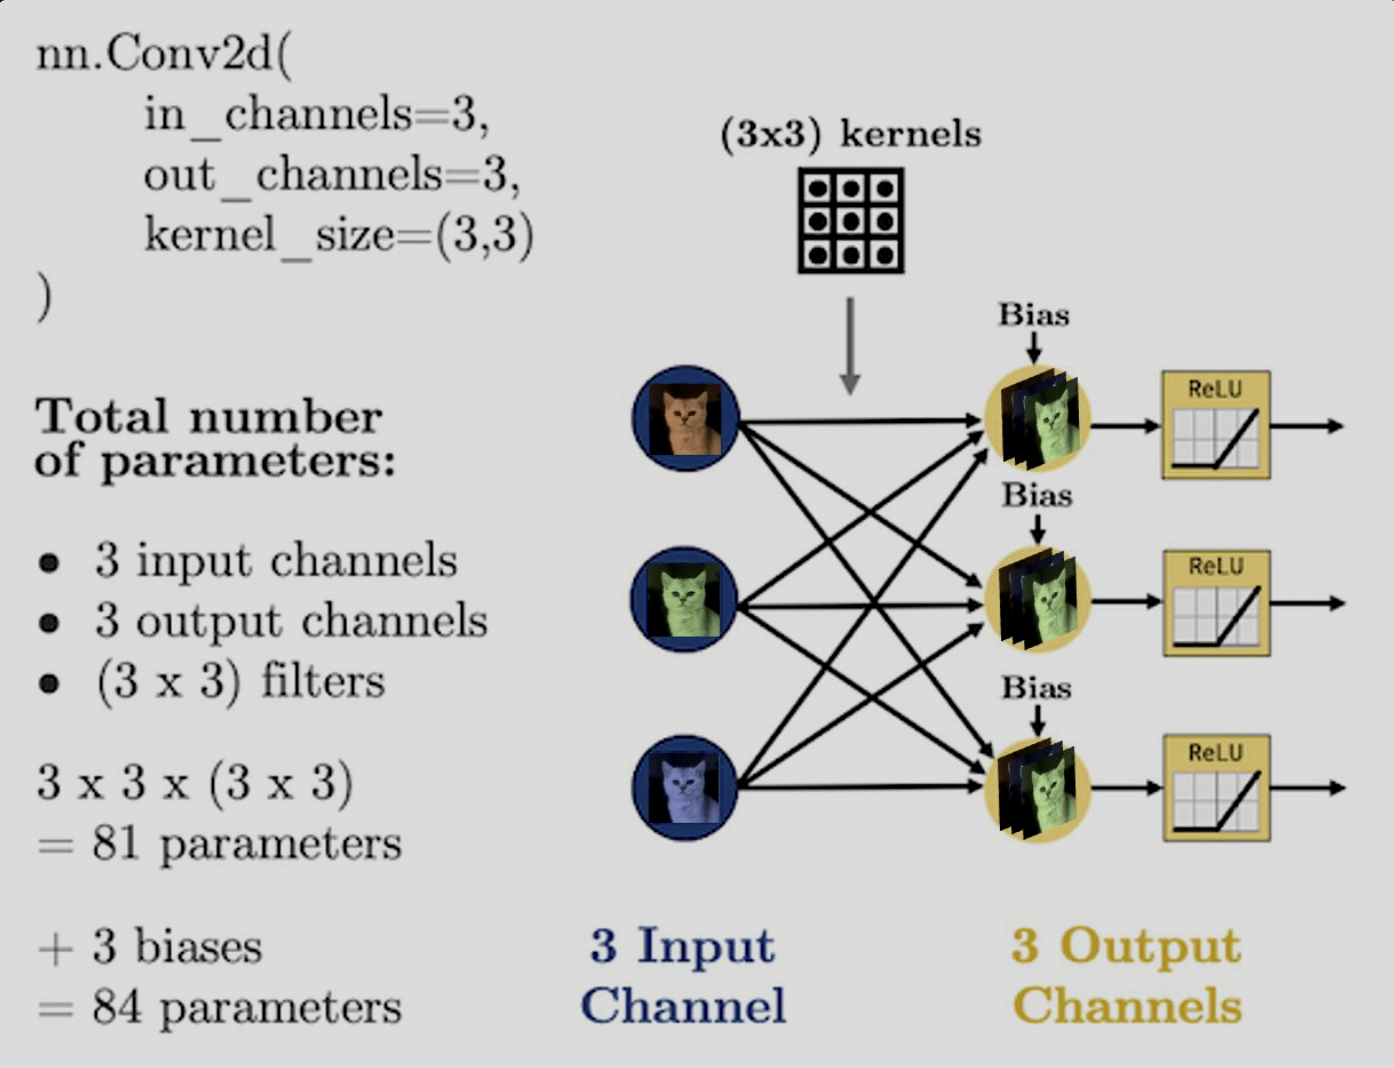
\includegraphics[width=0.5\linewidth, height=2cm]{CNN.png}
% 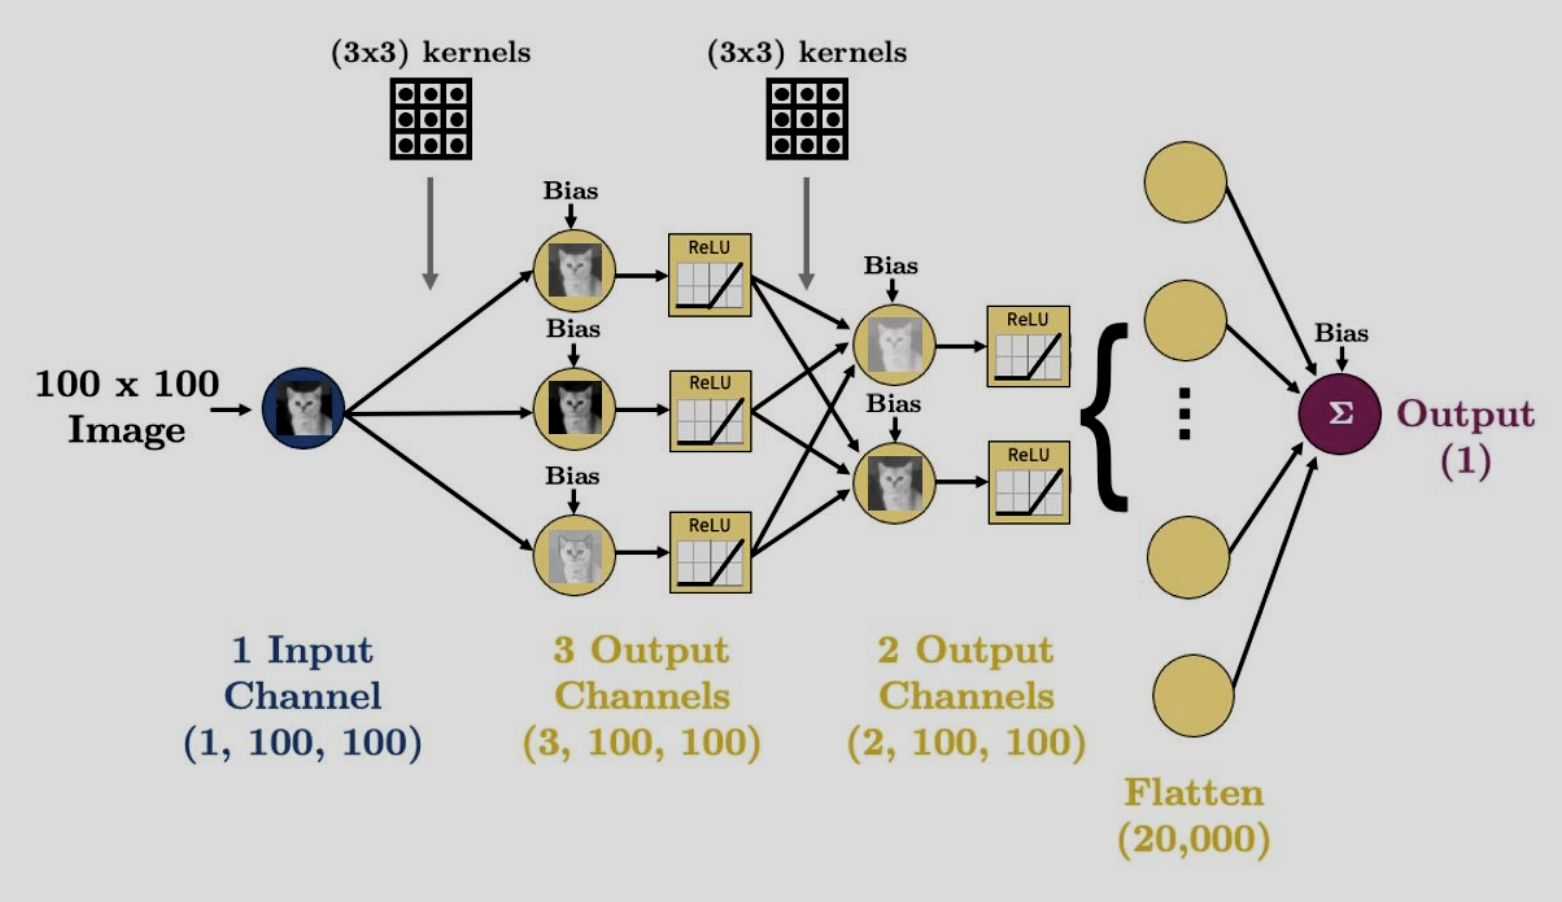
\includegraphics[width=0.5\linewidth, height=2cm]{flat.png}

\textbf{Flatten}
\smalltext{
    End of our network, we are going to need to torch.nn.Flatten() our images:
}
\textbf{Pooling}
\smalltext{
for reducing the dimensionality of the transformed images. max pooling or average pooling.
It derives the sharpest features of a transformed image.
}
\begin{lstlisting}[language=Python]
pool = nn.MaxPool2d(kernel_size=2, stride=2, padding=0)
x = torch.tensor([[[ 1.,  2., -1.,  0.],[ 3., -2.,  4.,  1.],
    [ 0.,  5.,  2., -3.],[ 1.,  1.,  7.,  2.],]])  # shape (1,1,4,4)
A = pool(x)
\end{lstlisting}
\smalltext{
Classification Problems: Output: class logits (size = classes) | Loss: CrossEntropyLoss | Metrics: accuracy, F1, etc. \\
Regression Problems: Output: one or more continuous values | Loss: often MSELoss | Metrics: MSE / RMSE / MAE (not acc)
}
\subsection{Data Augmentation}
\smalltext{
To make CNN more robust to variations like scaling or rotation, and to increase the diversity of your training data, either by generating variations dynamically or expanding the dataset size explicitly.
By applying data augmentation, we can expose the CNN to variations in the images, like rotations and flips, enabling it to learn and predict more effectively under these conditions. This helps the model generalize better to unseen data. Rotation/flipping/cropping/adding noise.
}
\subsection{Hyperparameter Tuning}
\smalltext{
    Number of layers. Number of nodes in each layer. Activation functions. Regularization. Initialization (starting weights). Optimization hyperparameters (learning rate, momentum, weight decay)
    Brute force strategies such as grid search perform poorly. 
    We can use an optimization algorithm instead of blindly evaluating our model for all values of hyperparameters.
    Ax uses Bayesian optimization to tune the hyperparameters. Ax is a black-box optimizer, which means we can ask it to optimize arbitray Python functions. 
}

\section{Transfer Learning}
\smalltext{
Instead, a common practice is to download a pre-trained model and fine tune it for your task. This is called transfer learning.
e.g.: AlexNet, VGG, ResNet, Inception, MobileNet, etc \\
\textbf{ImageNet} is an image dataset that became a very popular benchmark in the field ~10 years ago.
There are three common ways to use transfer learning in computer vision

\textbf{Feature extraction:}
freeze the pretrained backbone; train a small classifier head.
Pros: strong regularization, stable training, good for small datasets.

\textbf{Fine-tuning::}
unfreeze some/all backbone layers and train end-to-end.
Pros: can adapt features to your domain; Cons: can overfit/forget pretrained features, especially with small data or too-high LR.
}
\subsection{Using pre-trained models out-of-the-box}
\smalltext{
We got these predictions without “doing the ML ourselves”.
We are using pre-trained vgg16 model which is available in torchvision.
torchvision has many such pre-trained models available that have been very successful across a wide range of tasks: AlexNet, VGG, ResNet, Inception, MobileNet, etc.
}

\subsection{Using pre-trained models as feature extractors}
\smalltext{
1. Add some extra layers to the pre-trained network to suit our particular task.
}
\smalltext{
2. Pass training data through the network and save the output to use as features for training some other model
}


\begin{lstlisting}[language=Python]
densenet = models.densenet121(weights="DenseNet121_Weights.IMAGENET1K_V1")
for param in densenet.parameters():  # Freeze parameters
    param.requires_grad = False
densenet.classifier = nn.Identity()#remove last "classification"
Z_train, y_train, Z_valid, y_valid = get_features(
    densenet, dataloaders["train"], dataloaders["valid"]
)
\end{lstlisting}
    
\subsection{Using pre-trained models for fine tuning}
\smalltext{
Most common workflow of transfer learning.
Stacked some extra layers onto DenseNet and just trained those layer (we “froze” all of DenseNet's weights)
We can also “fine tune” DenseNet's weights if we like, to make it more suited to our data.    
}

\section{Yolo}
\smalltext{
Classification can be perfect while detection is poor (bad localization, missed objects).
Lower threshold gives more predicted boxes which means typically higher recall, lower precision but also includes more false positives.
YOLO outputs tensors (boxes + objectness + class scores). \\
High precision = few false alarms.
High recall = you miss few objects.
\textbf{Intersection-over-Union (IoU):}Metric that can be used to determine when two bounding boxes are locating the same object.
If the boxes cover regions A and B respectively, we define the intersection-over-union as: (A n B / A U B) Sometimes called “Jaccard index” or “Jaccard similarity”. [0,1].
Get \textbf{True positive} if the predicted label matches the ground truth label.
If we have Ground-truth box, but no prediction with IoU above the given threshold, we get a \textbf{false negative.}
A predicted box with no ground truth above IoU threshold is a \textbf{false positive}.
“Mean Average Precision” or “mAP”. We can calculate AP (area under PR curve) for each class independently; mAP is just the mean across all classes.
\textbf{Convolution layers downsample} They downsample.
\textbf{transposed convolution layers} They upsample.
}




\end{multicols}
\end{document}